\usetikzlibrary{arrows.meta}
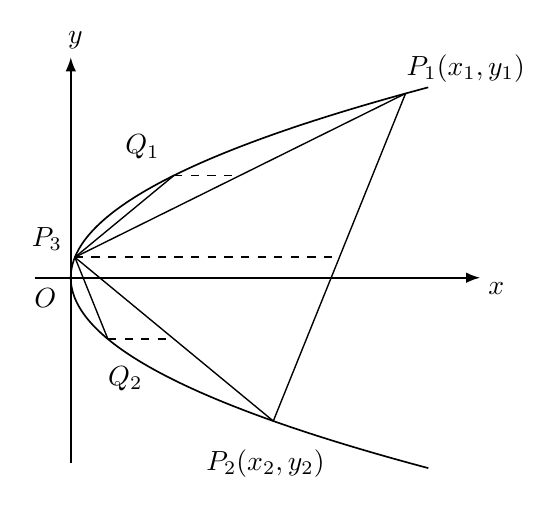
\begin{tikzpicture}[line width=.6pt,font=\normalsize,x=1cm,y=1cm]
\coordinate (P1) at (4.252,2.34);
\coordinate (P2) at (2.572,-1.82);
\coordinate (P3) at (0.052,0.26);
\coordinate (Q1) at (1.312,1.3);
\coordinate (Q2) at (0.472,-0.78);
\coordinate (M) at (3.413,0.26);
\coordinate (M1) at (2.152,1.3);
\coordinate (M2) at (1.312,-0.78);
% axes
\draw[-{Latex[length=1.8mm]}] (-0.45,0) -- (5.2,0);
\draw[-{Latex[length=1.8mm]}] (0,-2.35) -- (0,2.8);
% parabola y^2=2x, generated from the equation
\draw plot[domain=-4.65:4.65, samples=160] ({0.42*(\x*\x/2)},{0.52*\x});
% chords
\draw[line width=.5pt] (P3) -- (P1);
\draw[line width=.5pt] (P3) -- (P2);
\draw[line width=.5pt] (P1) -- (P2);
\draw[line width=.5pt] (P3)--(Q1);
\draw[line width=.5pt] (P3)--(Q2);
% horizontal construction lines
\draw[dashed] (P3) -- (M);
\draw[dashed] (Q1) -- (M1);
\draw[dashed] (Q2) -- (M2);
% labels
\node[anchor=south west, inner sep=1.5pt] at (4.202,2.42) {$P_1(x_1,y_1)$};
\node[anchor=north, inner sep=1.5pt] at (2.472,-2.12) {$P_2(x_2,y_2)$};
\node[anchor=south east, inner sep=1.5pt] at (-0.048,0.28) {$P_3$};
\node[anchor=south east, inner sep=1.5pt] at (1.192,1.44) {$Q_1$};
\node[anchor=north west, inner sep=1.5pt] at (0.412,-1.06) {$Q_2$};
\node[anchor=north east, inner sep=1.5pt] at (-0.12,-0.08) {$O$};
\node[anchor=west, inner sep=1.5pt] at (5.24,-0.14) {$x$};
\node[anchor=south, inner sep=1.5pt] at (0.06,2.84) {$y$};
\end{tikzpicture}
